\section{Auswertung}
\label{sec:Auswertung}

\begin{table}
    \centering
    \caption{Bestimmung der Schallgeschwindigkeit mittels Durchschallungs-Methode.}
    \label{tab:1}
    \sisetup{parse-numbers=false}
    \begin{tabular}{
	S[table-format=2.2]
	S[table-format=2.1]
	S[table-format=4.2]
	}
	\toprule
	{$h_{\text{zylinder}} \:/\: 10^{-3} \si{\metre}$}		& {$\increment t \:/\: 10^{-6} \si{\second} $}		& 
	{$c_\text{Acryl} \:/\: \si{\metre\per\second} $}		\\ 
	\midrule
    31.30 & 11.5 & 2709.96 \\
61.50 & 22.8 & 2697.37 \\
80.55 & 30.4 & 2645.32 \\

    \bottomrule
    \end{tabular}
    \end{table}


\input{build/Tabelle_2_texformat.tex}

\input{build/Tabelle_3_texformat.tex}

\input{build/Tabelle_4_texformat.tex}

\input{build/Tabelle_5_texformat.tex}

\input{build/Tabelle_6_texformat.tex}

\input{build/Tabelle_q_texformat.tex}

\input{build/Tabelle_q_neu_texformat.tex}

\begin{figure}
  \centering
  \includegraphics[height=8cm]{build/ladungen.pdf}
  \caption{Ermittelte Ladungen.}
  \label{plot:1}
\end{figure}

\begin{figure}
  \centering
  \includegraphics[height=8cm]{build/ladungen_neu.pdf}
  \caption{Korrigierte Ladungen.}
  \label{plot:2}
\end{figure}

\begin{align*}
  e_0 = \input{build/e_0.tex}
\end{align*}

\begin{align*}
  e_{0,\text{neu}} = \input{build/e_0_neu.tex}
\end{align*}

\begin{align*}
  N_{a} = \input{build/N_a.tex}
\end{align*}

\begin{align*}
  N_{a,\text{neu}} = \input{build/N_a_neu.tex}
\end{align*}



% % Examples
% \begin{equation}
%   U(t) = a \sin(b t + c) + d
% \end{equation}
%
% \begin{align}
%   a &= \input{build/a.tex} \\
%   b &= \input{build/b.tex} \\
%   c &= \input{build/c.tex} \\
%   d &= \input{build/d.tex} .
% \end{align}
% Die Messdaten und das Ergebnis des Fits sind in Abbildung~\ref{fig:plot} geplottet.
%
% %Tabelle mit Messdaten
% \begin{table}
%   \centering
%   \caption{Messdaten.}
%   \label{tab:data}
%   \sisetup{parse-numbers=false}
%   \begin{tabular}{
% % format 1.3 bedeutet eine Stelle vorm Komma, 3 danach
%     S[table-format=1.3]
%     S[table-format=-1.2]
%     @{${}\pm{}$}
%     S[table-format=1.2]
%     @{\hspace*{3em}\hspace*{\tabcolsep}}
%     S[table-format=1.3]
%     S[table-format=-1.2]
%     @{${}\pm{}$}
%     S[table-format=1.2]
%   }
%     \toprule
%     {$t \:/\: \si{\milli\second}$} & \multicolumn{2}{c}{$U \:/\: \si{\kilo\volt}$\hspace*{3em}} &
%     {$t \:/\: \si{\milli\second}$} & \multicolumn{2}{c}{$U \:/\: \si{\kilo\volt}$} \\
%     \midrule
%     \input{build/table.tex}
%     \bottomrule
%   \end{tabular}
% \end{table}
%
% % Standard Plot
% \begin{figure}
%   \centering
%   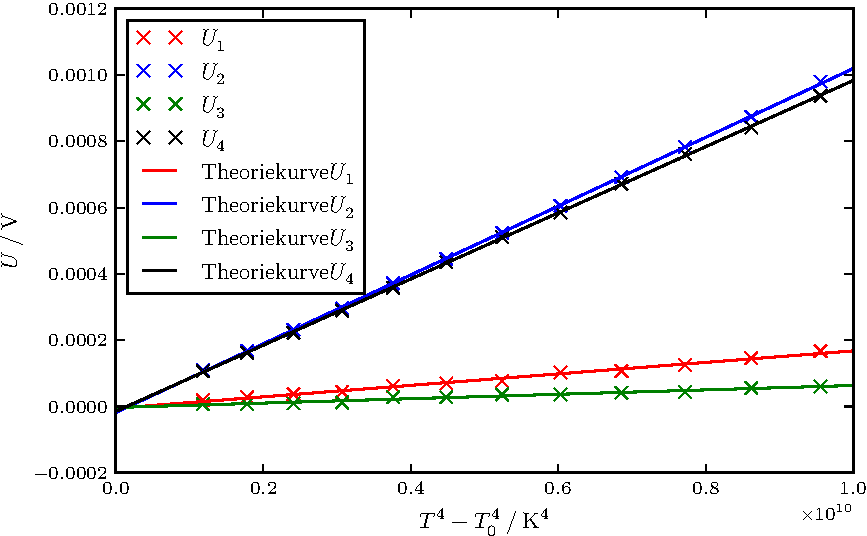
\includegraphics{build/plot.pdf}
%   \caption{Messdaten und Fitergebnis.}
%   \label{fig:plot}
% \end{figure}
%
% 2x2 Plot
% \begin{figure*}
%     \centering
%     \begin{subfigure}[b]{0.475\textwidth}
%         \centering
%         \includegraphics[width=\textwidth]{Abbildungen/Schaltung1.pdf}
%         \caption[]%
%         {{\small Schaltung 1.}}
%         \label{fig:Schaltung1}
%     \end{subfigure}
%     \hfill
%     \begin{subfigure}[b]{0.475\textwidth}
%         \centering
%         \includegraphics[width=\textwidth]{Abbildungen/Schaltung2.pdf}
%         \caption[]%
%         {{\small Schaltung 2.}}
%         \label{fig:Schaltung2}
%     \end{subfigure}
%     \vskip\baselineskip
%     \begin{subfigure}[b]{0.475\textwidth}
%         \centering
%         \includegraphics[width=\textwidth]{Abbildungen/Schaltung4.pdf}    % Zahlen vertauscht ... -.-
%         \caption[]%
%         {{\small Schaltung 3.}}
%         \label{fig:Schaltung3}
%     \end{subfigure}
%     \quad
%     \begin{subfigure}[b]{0.475\textwidth}
%         \centering
%         \includegraphics[width=\textwidth]{Abbildungen/Schaltung3.pdf}
%         \caption[]%
%         {{\small Schaltung 4.}}
%         \label{fig:Schaltung4}
%     \end{subfigure}
%     \caption[]
%     {Ersatzschaltbilder der verschiedenen Teilaufgaben.}
%     \label{fig:Schaltungen}
% \end{figure*}
